%%%%%%%%%%%%%%%%%%%%%%%%%%%%%%%%%%%%%%%%%%%%%%%%%%%%%%%%%%%%%%%%%%%%%%%%%%%%
% AGUJournalTemplate.tex: this template file is for articles formatted with LaTeX
%
% This file includes commands and instructions
% given in the order necessary to produce a final output that will
% satisfy AGU requirements, including customized APA reference formatting.
%
% You may copy this file and give it your
% article name, and enter your text.
%
%
% Step 1: Set the \documentclass
%
%

%% To submit your paper:
%\documentclass[draft]{agujournal2019}
%\usepackage{url} 
%\usepackage{graphicx,natbib,overpic,xcolor}
%\usepackage{apacite}
%\bibliographystyle{unsrtnat}
%this package should fix any errors with URLs in refs.
%\usepackage{lineno}
\usepackage{geometry}
%\usepackage[inline]{trackchanges} %for better track changes. finalnew option will compile document with changes incorporated.
%\usepackage{soul}
%\linenumbers

\documentclass[draft,linenumbers]{agujournal2019}
\usepackage{apacite}
\usepackage{url} %this package should fix any errors with URLs in refs.
\usepackage{enumitem}
\usepackage{amsmath}
\usepackage{overpic}
\usepackage{pict2e}
\usepackage{bm}
%%%%%%%


\draftfalse

%% Enter journal name below.
%% Choose from this list of Journals:
%
% JGR: Atmospheres
% JGR: Biogeosciences
% JGR: Earth Surface
% JGR: Oceans
% JGR: Planets
% JGR: Solid Earth
% JGR: Space Physics
% Global Biogeochemical Cycles
% Geophysical Research Letters
% Paleoceanography and Paleoclimatology
% Radio Science
% Reviews of Geophysics
% Tectonics
% Space Weather
% Water Resources Research
% Geochemistry, Geophysics, Geosystems
% Journal of Advances in Modeling Earth Systems (JAMES)
% Earth's Future
% Earth and Space Science
% Geohealth
%
% ie, \journalname{Water Resources Research}

\journalname{Diurnal Aggregation}


\begin{document}

%% ------------------------------------------------------------------------ %%
%  Title
%
% (A title should be specific, informative, and brief. Use
% abbreviations only if they are defined in the abstract. Titles that
% start with general keywords then specific terms are optimized in
% searches)
%
%% ------------------------------------------------------------------------ %%

% Example: \title{This is a test title}

\title{Diurnal Self-Aggregation}

%% ------------------------------------------------------------------------ %%
%
%  AUTHORS AND AFFILIATIONS
%
%% ------------------------------------------------------------------------ %%

% Authors are individuals who have significantly contributed to the
% research and preparation of the article. Group authors are allowed, if
% each author in the group is separately identified in an appendix.)

% List authors by first name or initial followed by last name and
% separated by commas. Use \affil{} to number affiliations, and
% \thanks{} for author notes.
% Additional author notes should be indicated with \thanks{} (for
% example, for current addresses).

% Example: \authors{A. B. Author\affil{1}\thanks{Current address, Antartica}, B. C. Author\affil{2,3}, and D. E.
% Author\affil{3,4}\thanks{Also funded by Monsanto.}}

\authors{Jan O. Haerter}


% \affiliation{1}{First Affiliation}
% \affiliation{2}{Second Affiliation}
% \affiliation{3}{Third Affiliation}
% \affiliation{4}{Fourth Affiliation}

\affiliation{1}{Niels Bohr Institute, University of Copenhagen, Blegdamsvej 17, 2100 Copenhagen, Denmark}
%(repeat as many times as is necessary)

%% Corresponding Author:
% Corresponding author mailing address and e-mail address:

% (include name and email addresses of the corresponding author.  More
% than one corresponding author is allowed in this LaTeX file and for
% publication; but only one corresponding author is allowed in our
% editorial system.)

% Example: \correspondingauthor{First and Last Name}{email@address.edu}

\correspondingauthor{Jan O. Haerter}{haerter@nbi.ku.dk}

%% Keypoints, final entry on title page.

%  List up to three key points (at least one is required)
%  Key Points summarize the main points and conclusions of the article
%  Each must be 100 characters or less with no special characters or punctuation and must be complete sentences

% Example:
% \begin{keypoints}
% \item	List up to three key points (at least one is required)
% \item	Key Points summarize the main points and conclusions of the article
% \item	Each must be 100 characters or less with no special characters or punctuation and must be complete sentences
% \end{keypoints}

\begin{keypoints}
\item Self-aggregation is possible within short timeperiods, when boundary conditions oscillate,
\item the effect is nearly independent of domain size or resolution,
\item the effect requires only moderate temperature amplitudes.
\end{keypoints}

%% ------------------------------------------------------------------------ %%
%
%  ABSTRACT and PLAIN LANGUAGE SUMMARY
%
% A good Abstract will begin with a short description of the problem
% being addressed, briefly describe the new data or analyses, then
% briefly states the main conclusion(s) and how they are supported and
% uncertainties.

% The Plain Language Summary should be written for a broad audience,
% including journalists and the science-interested public, that will not have 
% a background in your field.
%
% A Plain Language Summary is required in GRL, JGR: Planets, JGR: Biogeosciences,
% JGR: Oceans, G-Cubed, Reviews of Geophysics, and JAMES.
% see http://sharingscience.agu.org/creating-plain-language-summary/)
%
%% ------------------------------------------------------------------------ %%

%% \begin{abstract} starts the second page

\begin{abstract}
Convective self-aggregation is a paradigm for tropical oceanic cloud organization \cite{wing2017convective} and has been shown to give rise to cloud clusters over timescales of weeks\cite{khairoutdinov2010aggregation,muller2012detailed}.
In contrast to the standard radiative convective equilibrium setup \cite{held1993radiative,tompkins1998radiative}, where surface conditions are held constant, we here allow surface conditions to oscillate diurnally, but allow the system to reach a repetitive state, termed perpetual equilibrium \cite{schlemmer2011diurnal,haerter2018intensified}.
While the atmosphere gradually equilibrates at the system scale and domain mean precipitation indeed becomes similar from day to day, the spatial distribution of precipitation is only homogeneous during the first day. 
Already during the second day, the precipitation field is strongly structured and continues to cluster in subsequent days.
The clustering is robust to changes in resolution but can be removed by reduction of the amplitude of oscillation.
Our results suggest that a modest diurnal cycle in forcing conditions can lead to aggregation-like structuring of the convective atmosphere.
The results may help clarify, how cloud clustering in the tropics could arise much more rapidly than through conventional self-aggregation.
\end{abstract}

\section*{Plain Language Summary}
[ enter your Plain Language Summary here or delete this section]


%% ------------------------------------------------------------------------ %%
%
%  TEXT
%
%% ------------------------------------------------------------------------ %%

%%% Suggested section heads:
% \section{Introduction}
%
% The main text should start with an introduction. Except for short
% manuscripts (such as comments and replies), the text should be divided
% into sections, each with its own heading.

% Headings should be sentence fragments and do not begin with a
% lowercase letter or number. Examples of good headings are:

% \section{Materials and Methods}
% Here is text on Materials and Methods.
%
% \subsection{A descriptive heading about methods}
% More about Methods.
%
% \section{Data} (Or section title might be a descriptive heading about data)
%
% \section{Results} (Or section title might be a descriptive heading about the
% results)
%
% \section{Conclusions}


\section{Introduction}\label{sec:intro}
As an idealized numerical description of tropical convective self-organization, self-aggregation, where the cloud field segregates into cloudy and less cloudy sub-domains, usually assumes spatially and temporally constant surface moisture (sea surface) and temperature ($\sim 300\;K$) \cite{muller2012detailed}.
It is well-known that many factors influence self-aggregation, such as sea surface temperature and surface feedbacks \cite{hohenegger2016coupled}, domain size, geometry and resolution \cite{muller2015favors}, as well as cold pool effects \cite{jeevanjee2013convective,haerter2019convective}.
Above all, radiation feedbacks have however emerged as the "smoking gun" for sustaining and increasing the inequality between the sub-regions \cite{bretherton2005energy}.
It has been argued, that cloudy regions --- which benefit from warming cloud feedbacks --- tend to emit less heat to space than do cloud-free regions.
Together, these two effects induce net near-surface divergence from cloud-free regions and convergence into already cloudy ones --- bringing more moisture into cloudy regions, thus further enhancing the imbalance.

Whereas numerical simulations assume constant insolation as well as surface boundary conditions, buoy-based instruments do measure diurnal variations in tropical sea surface temperature by typically 0.5-2 K \cite{weller1996surface,johnson1999trimodal} and satellite observations show a diurnal cycle in cloud height for the Madden Julian Oscillation \cite{suzuki2009diurnal,tian2006modulation}.
Diurnal cycles in precipitation also emerge from two-dimensional numerical simulations where variations in insolation are accounted for \cite{liu1998numerical}. 
This and earlier studies\cite{chen1997diurnal} also describe a persistent organized state of a mesoscale convective system, with characteristics of a squall line.
\cite{chen1997diurnal} find a dynamics referred to as "diurnal dancing", which involves a bi-diurnal oscillation of local cloudiness.
\cite{guichard2004modelling,brown2002large,petch2002impact,schlemmer2011diurnal,moseley2016,haerter2018intensified}, as simulated domains show typical build-up on convective available potential energy during the morning hours, and its release in terms of precipitation during the afternoon or evening.
Yet, as the focus was often on the timing or the overall intensity of rainfall, simulated domains were either chosen to be relatively small and model resolutions relatively high. 
State-of-the-art regional climate models now simulate relatively large domains ($\sim 1000$ $km$ at $1$ or $2$ $\;km$ resolution), but include the full complexity of the lateral forcing \cite{ban2015heavy}. 

Sahelian MCS \cite{mathon2001life}
Sea surface impact atmosphere \cite{kawai2007diurnal}
2day equatorial waves \cite{haertel2004dynamics}
scale interaction MJO diurnal cycle \cite{peatman2014propagation}
tropical precipitation extremes and mesoscale systems \cite{rossow2013tropical}
Rich gets richer effect \cite{chou2009evaluating}

\section{Methods}\label{sec:methods}
We simulate the convective atmosphere using the University of California, Los Angeles (UCLA) Large Eddy Simulation (LES) model with sub-grid scale turbulence parameterized after Smagorinsky \cite{smagorinsky1963general}, a delta four-stream radiation scheme \cite{pincus} and a two-moment cloud microphysics scheme \cite{stevens2005}. 
Rain evaporation is implemented after \citet{seifert2006two}.
As detailed in \cite{moseley2016}, diurnally oscillating surface temperature ($T_s(t)$) boundary conditions are applied, with
\begin{eqnarray}
  T_s(t)=\overline{T_{s}}-T_{a} \cos{(2\pi\;t/t_0)}\;,
\end{eqnarray}
\noindent
with $\overline{T_{s}}=298\;K$ and $t_0=24\;h$ is the duration of the simulated model day.
All simulations were initialized with data from observed summertime mid-latitude conditions where convection had occurred in order to establish an initially unstable atmosphere. 
However, due to the repeated diurnal cycle forcing, the system eventually establishes a self-consistent vertical temperature and moisture profile [show this somewhere].

\noindent
The model numerically integrates the anelastic equations of motion on a regular horizontal domain with varying horizontal grid spacing $dx$ and periodic boundary conditions. 
The model spans 75 stretchable vertical levels peaking at the full domain height of 16.5 km with a sponge layer above 12.3 km.
The Coriolis force and the mean wind were set to zero with weak random initial perturbations added as noise to break complete spatial symmetry. 
No large scale forcing was imposed,
ensuring that the only driving force for convection was buoyancy and the forced lifting through cold pool interaction.
The model output time step is $\Delta t_{out}=5\;min$. 
At each output time step, instantaneous precipitation intensity, moisture and velocity fields are output at each model gridbox. 

We carry out a range of distinct simulations:
\begin{table}
    \centering
    \begin{tabular}{c|c|c|c}
        Experiment & Surface Temperature Amplitude, $T_a$ & Horizontal Resolution, $dx$ & Domain Size, $L$\\
        A & 5 & 1 & 500\\
    \end{tabular}
    \caption{Summary of numerical experiments}
    \label{tab:experiments_overview}
\end{table}

\begin{itemize}
    \item {\bf A}: $T_a=5\;K$ and $dx=1\;km$,
    \item {\bf B}: $T_a=2\;K$ and $dx=1\;km$,
    \item {\bf C}: $T_a=5\;K$ and $dx=.5\;km$.
\end{itemize}


\section{Results}\label{sec:results}

\subsection{Domain mean timeseries}

\subsection{Characterizing the active and quiescent phases}

\subsection{Characterizing the dynamics}


\begin{figure*}
\centering
%\begin{overpic}
%\includegraphics[height=0.33\linewidth]{cavities}
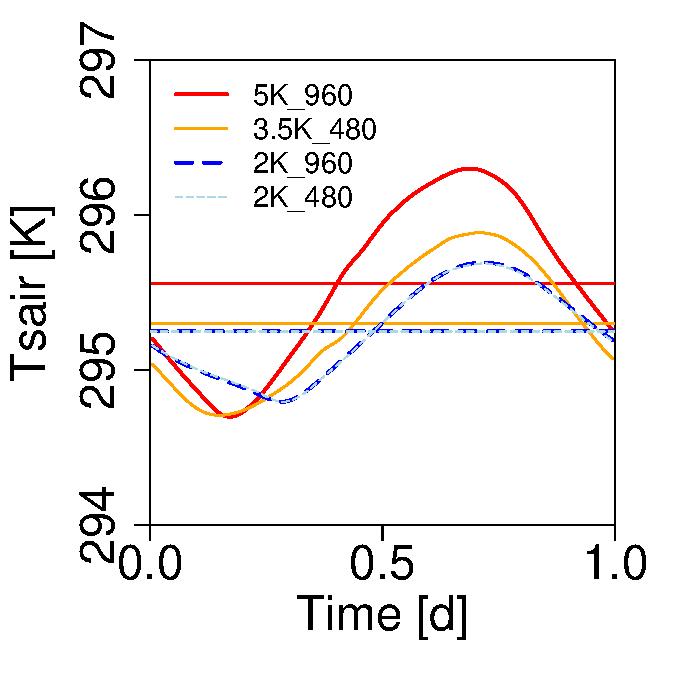
\includegraphics[trim={0 0 0cm 0}, clip, height=0.32\linewidth]{tsair_varying_ampl_timeseries_agg.pdf}
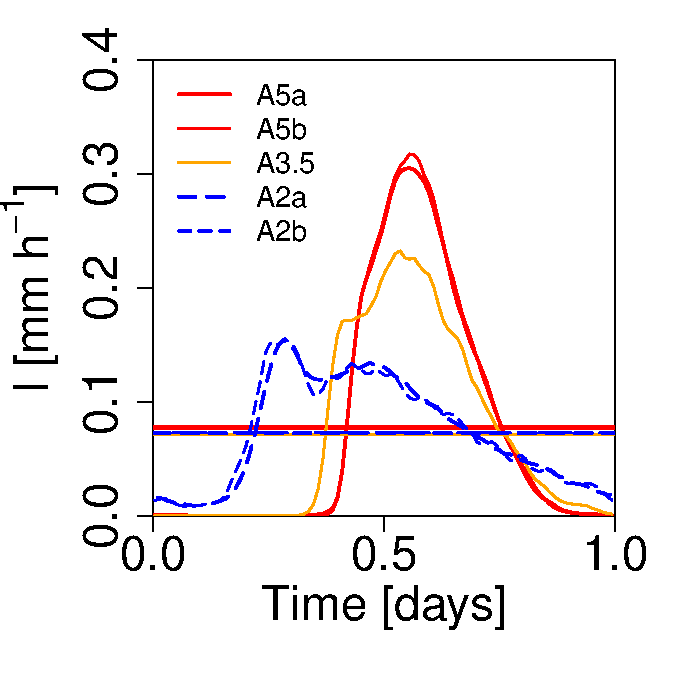
\includegraphics[trim={0 0 0cm 0}, clip, height=0.32\linewidth]{prcp_varying_ampl_timeseries_agg.pdf}
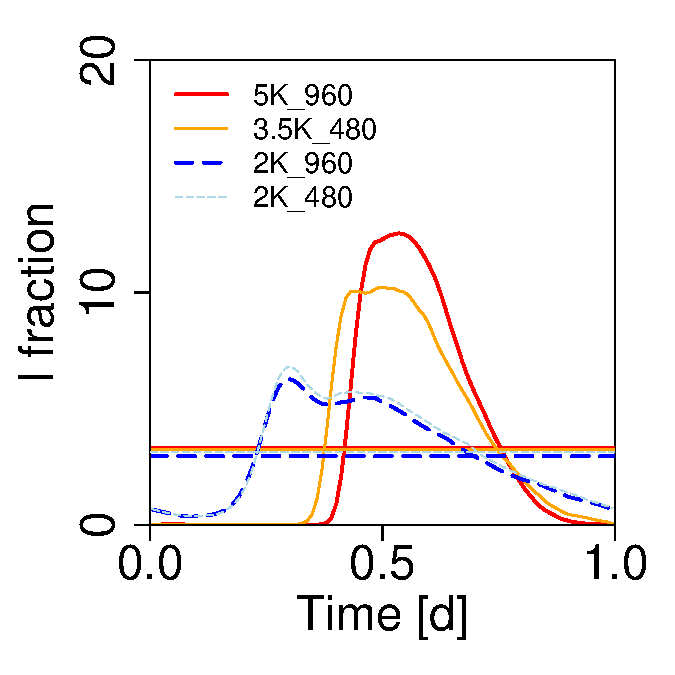
\includegraphics[trim={0 0 0cm 0}, clip, height=0.32\linewidth]{pfrac_varying_ampl_timeseries_agg.pdf}
\caption{{\bf Diurnal cycles of domain averaged quantities}. 
Each quantity was averaged over the spatial model domain. The timeseries is a compound diurnal cycle, where equal times of day were averaged over all available model days.
{\bf a}, Near-surface temperature for simulations with different imposed surface temperature amplitudes, as labeled in legend. Horizontal lines of corresponding colors represent the time average of each simulation.
{\bf b}, Analogous to (a), but for rain intensity.
{\bf c}, Analogous to (a), but for rain area fraction. 
}
\label{fig:domain_mean_timeseries}
\end{figure*}

\begin{figure*}
\centering
\begin{overpic}[width=0.4\textwidth ]{dummy.pdf}
\put(-70,40){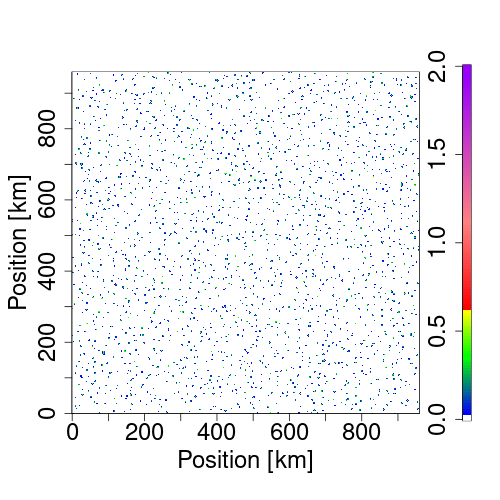
\includegraphics[height=0.38\linewidth,trim=0cm 2.75cm 2.6cm 0cm, clip]{var1_daymean_T0_300K_ampl_4_1km_large_1-96.png}}
\put(0,40){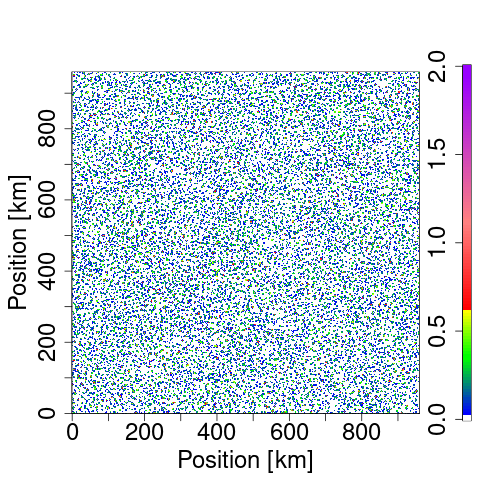
\includegraphics[trim={2.4cm 2.75cm 2.6cm 0cm}, clip, height=0.38\linewidth]{var1_daymean_T0_300K_ampl_4_1km_large_289-384.png}}
\put(60,40){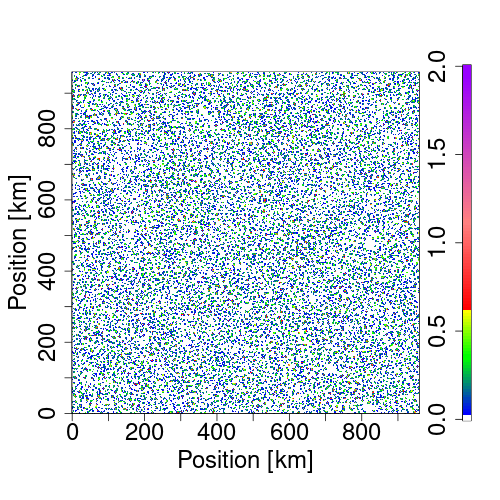
\includegraphics[trim={2.4cm 2.75cm 0cm 0cm}, clip, height=0.38\linewidth]{var1_daymean_T0_300K_ampl_4_1km_large_385-480.png}}
\put(-70,-35){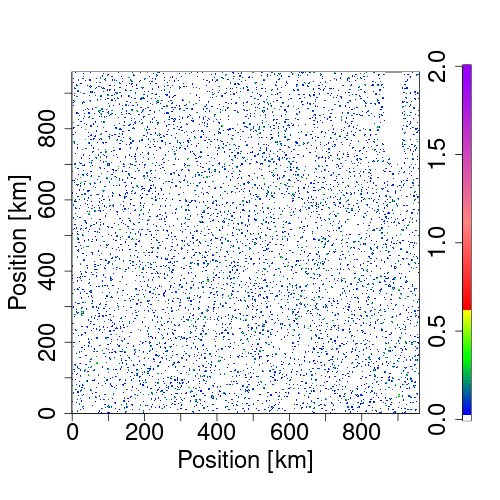
\includegraphics[trim={0cm 0cm 2.6cm 1.75cm}, clip, height=0.4\linewidth]{var1_daymean_T0_300K_ampl_10_1km_large_1-144.png}}
\put(0,-35){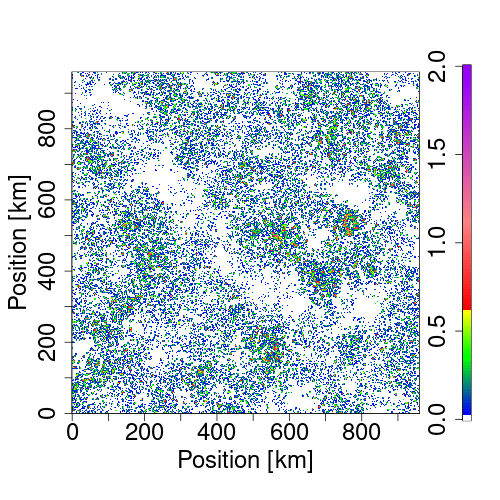
\includegraphics[trim={2.4cm 0cm 2.6cm 1.75cm}, clip, height=0.4\linewidth]{var1_daymean_T0_300K_ampl_10_1km_large_433-576.png}}
\put(60,-35){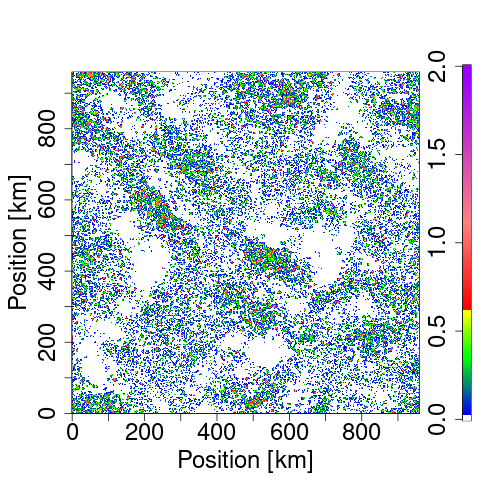
\includegraphics[trim={2.4cm 0cm 2.6cm 1.75cm}, clip, height=0.4\linewidth]{var1_daymean_T0_300K_ampl_10_1km_large_577-720.png}}
\put(-62,97){\large \bf a}
\put(-2,97){\large \bf b}
\put(59,97){\large \bf c}
\put(-62,34){\large \bf d}
\put(-2,34){\large \bf e}
\put(59,34){\large \bf f}
\end{overpic}
\vspace{2cm}
\caption{{\bf Transition to a clustered rainfall state.}
{\bf a}, Surface rainfall average during the first day (spin up) for $\Delta T=2\;K$.
{\bf b}, Similar to (a), but for day 3.
{\bf c}, Similar to (a), but for day 4.
{\bf d---f}, Similar to (a)---(c), but for $\Delta T=5\;K$.
}
\label{fig:daily_sum_5K}
\end{figure*}



\begin{figure}
\centering
\begin{overpic}[width=0.4\textwidth ]{dummy.pdf}
\put(-60,0){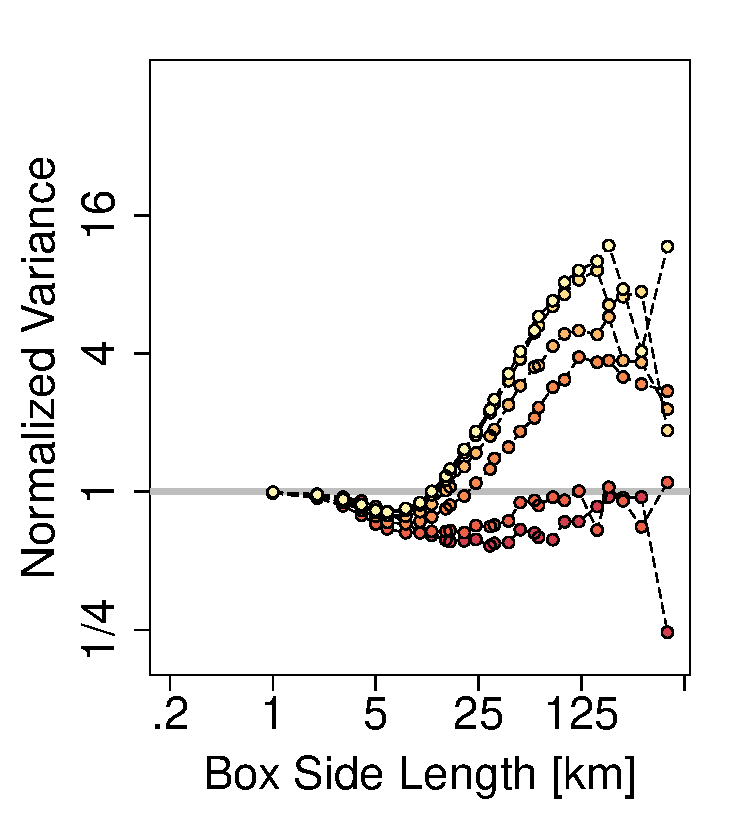
\includegraphics[trim={0cm 0cm 0cm 0cm}, clip, height=0.5\linewidth]{var_5K_960.pdf}}
\put(10,0){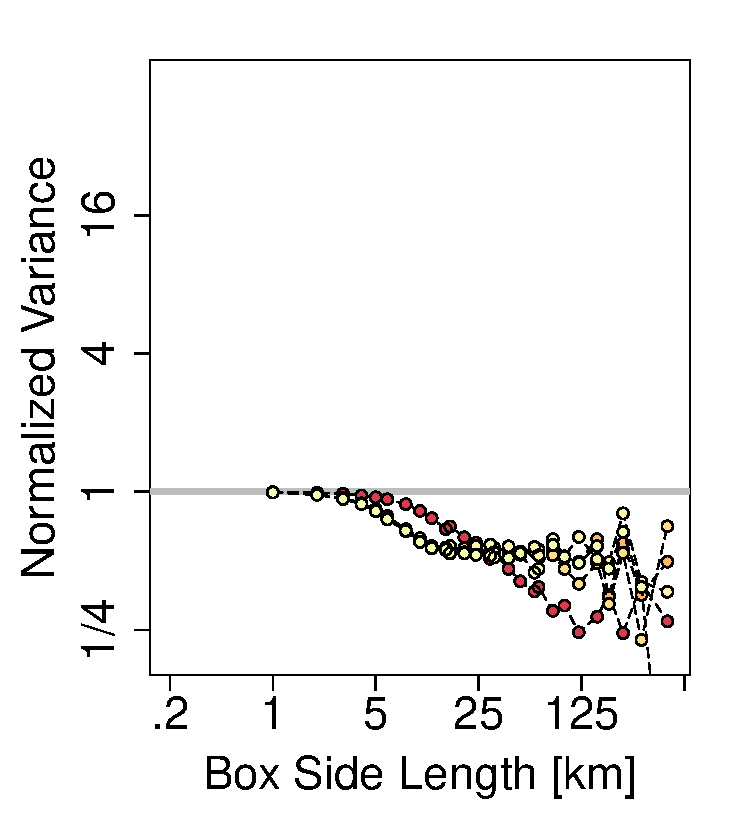
\includegraphics[trim={2cm 0cm 0cm 0cm}, clip, height=0.5\linewidth]{var_2K_960.pdf}}
\put(60,0){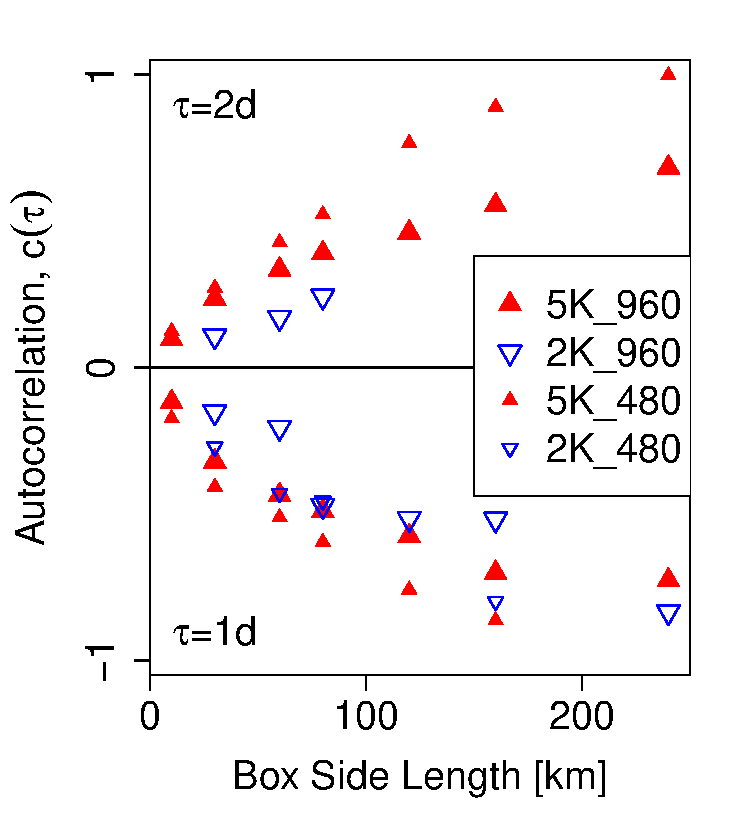
\includegraphics[trim={0cm 0cm 0cm 0cm}, clip, height=0.5\linewidth]{autocor_vs_day.pdf}}
%\put(-70,40){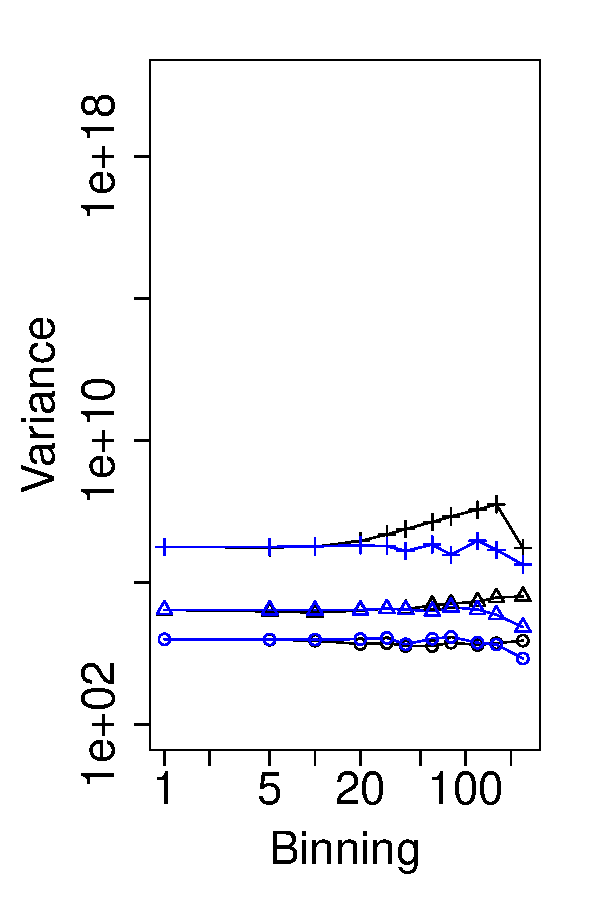
\includegraphics[trim={2cm 0cm 0cm 0cm}, clip, height=0.5\linewidth]{var_ampl_10K_480_500m.pdf}}
\end{overpic}
\caption{{\bf Spatial variance for different simulations at different times.}. 
{\bf a}---{\bf d}, $\Delta T=10\;K$, $480km\times 480km$, $\Delta x=1\;km$; same as (a) but $960km\times 960km$; same as (a) but $\Delta x=500\;m$; same as (a) but $\Delta T=4\;K$.
}
\label{fig:daily_sum_500m}
\end{figure}

\section{Discussion}\label{sec:discussions}

\section{Conclusion}\label{sec:conclusion}


\acknowledgments
JOH gratefully acknowledges funding by a grant from the VILLUM Foundation (grant number: 13168) and the European Research Council (ERC) under the European Union's Horizon 2020 research and innovation program (grant number: 771859).
The authors are grateful for computing resources and technical assistance provided by the Danish Center for Climate Computing, a facility built with support of the Danish e-Infrastructure Corporation, Danish Hydrocarbon Research and Technology Centre, VILLUM Foundation, and the Niels Bohr Institute.

\bibliography{references_clustering}



%Reference citation instructions and examples:
%
% Please use ONLY \cite and \citeA for reference citations.
% \cite for parenthetical references
% ...as shown in recent studies (Simpson et al., 2019)
% \citeA for in-text citations
% ...Simpson et al. (2019) have shown...
%
%
%...as shown by \citeA{jskilby}.
%...as shown by \citeA{lewin76}, \citeA{carson86}, \citeA{bartoldy02}, and \citeA{rinaldi03}.
%...has been shown \cite{jskilbye}.
%...has been shown \cite{lewin76,carson86,bartoldy02,rinaldi03}.
%... \cite <i.e.>[]{lewin76,carson86,bartoldy02,rinaldi03}.
%...has been shown by \cite <e.g.,>[and others]{lewin76}.
%
% apacite uses < > for prenotes and [ ] for postnotes
% DO NOT use other cite commands (e.g., \citet, \citep, \citeyear, \nocite, \citealp, etc.).
%


\begin{figure}
\centering
%\begin{overpic}
%\includegraphics[height=0.33\linewidth]{cavities}
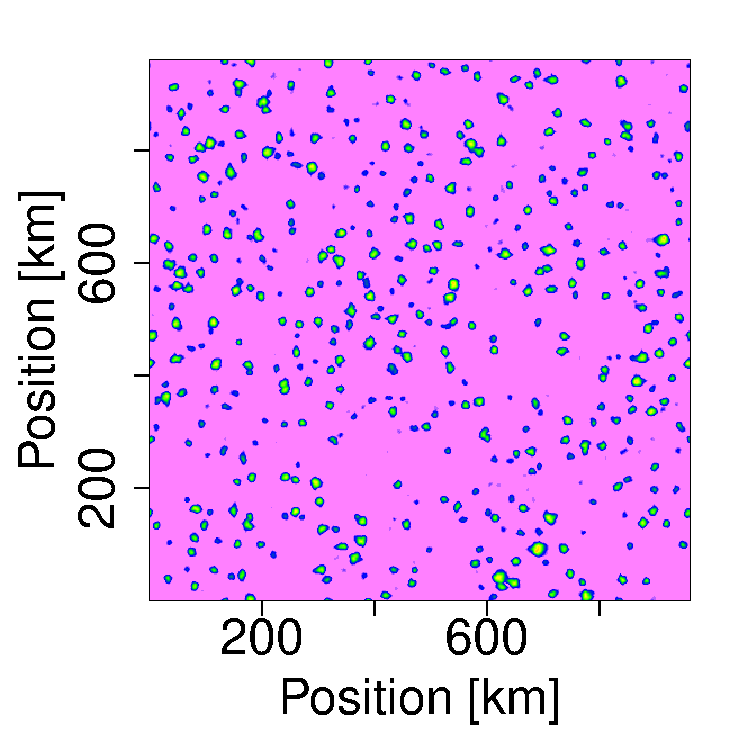
\includegraphics[trim={2cm 2.4cm 1cm 1cm}, clip, height=0.11\linewidth]{1-288_T0_300K_ampl_10_500m_r_int_timmean_xy_plot_l=2.pdf}
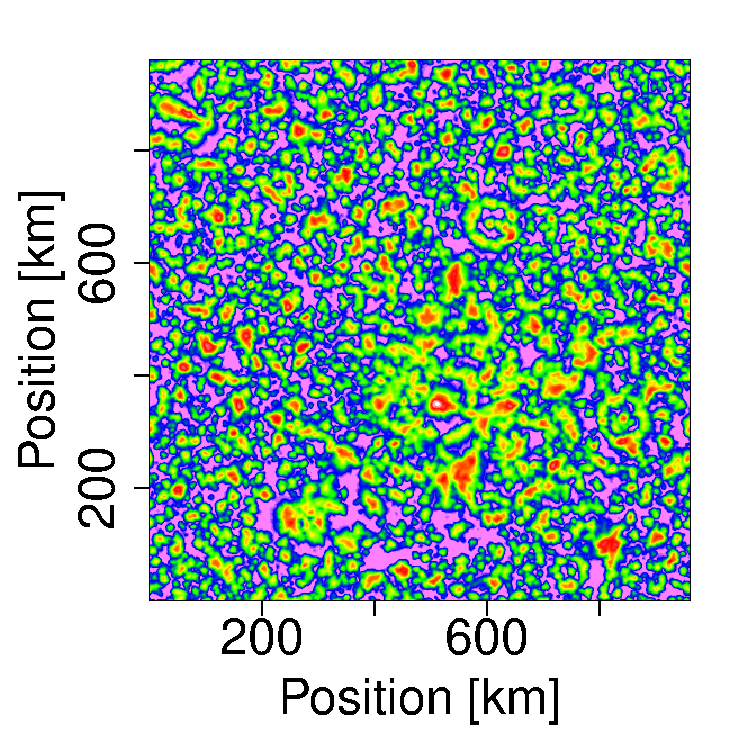
\includegraphics[trim={2cm 2.4cm 1cm 1cm}, clip, height=0.11\linewidth]{289-576_T0_300K_ampl_10_500m_r_int_timmean_xy_plot_l=2.pdf}
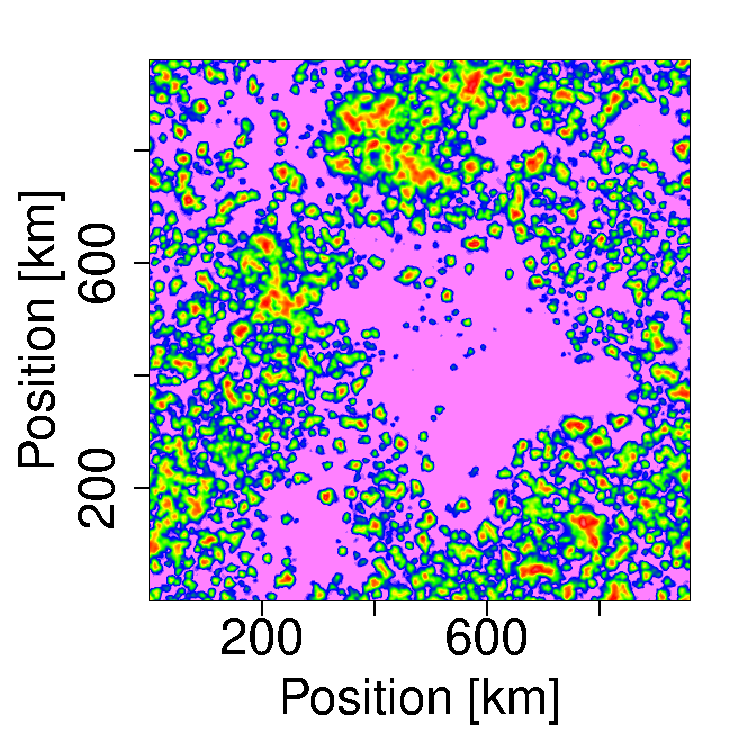
\includegraphics[trim={2cm 2.4cm 1cm 1cm}, clip, height=0.11\linewidth]{577-864_T0_300K_ampl_10_500m_r_int_timmean_xy_plot_l=2.pdf}
\caption{{\bf Daily precipitation sum for higher lateral model resolution.}. }
\label{fig:daily_sum_500m}
\end{figure}


\end{document}

